\documentclass[10pt]{paper}
\usepackage[a4paper, total={6in, 9in}, bottom = 1in]{geometry}
\usepackage[utf8]{inputenc}
\usepackage[slovak]{babel}
\usepackage{fancyhdr}
\usepackage{mathtools}
\usepackage{pgfplots}
\usepackage{wrapfig}
\usepackage{amsmath}
\usepackage{algpseudocode}
\newcommand{\name}{Katarína Kejstová 433820, Viktória Vozárová 433334}
\newcommand{\datum}{Projekt IV109}
\pagestyle{fancy}
\fancyhf{}
\lhead{\name}
\rhead{\datum}
\begin{document}

\begin{titlepage}
\begin{center}
  \bfseries
  \huge Záverečná správa
  \vskip.2in
  \textsc{\LARGE Projektu IV109 }
  \vskip1in
  \emph{\huge Robot - zbieranie pokladu}
\end{center}

\vskip1.4in

\begin{minipage}{.25\textwidth}
  \begin{flushleft}
    \bfseries\large Prednášajúci:\par \emph{doc. Mgr. Radek Pelánek, Ph.D.}
  \end{flushleft}
\end{minipage}
\hskip.4\textwidth
\begin{minipage}{.25\textwidth}
  \begin{flushleft}
    \bfseries\large Študenti:\par \emph{Katarína Kejstová} 433820 \par \emph{Viktória Vozárová} 422224
  \end{flushleft}
\end{minipage}

\vskip1.3in

\centering
\bfseries
\Large letný semester 2016
\end{titlepage}

\section{Zadanie}

Variace na příklad zmíněný na přednášce. Robot se pohybuje v čtvercové mřížce, na některých polích jsou poklady, které má posbírat, případně zdi, díry, a pod. Vytvořte genetický algoritmus, který bude vytvářet navigační kód pro robota (tak aby posbíral co nejvíce pokladu).


stručné uvedení do tématu, objasnění základních pojmů,
přesnou formulaci modelovaného problému, případná relevantní data,
popis zvoleného přístupu k modelování a základních prvků modelu, vztahů a zpětných vazeb, vysvětlení základních rovnic/pravidel,
popis výsledků simulace, ilustrace základního běhu modelu,
popis provedených analýz modelu (analýza citlivosti jednotlivých parametrů, apd), výsledky analýz a jejich slovní interpretace,
zhodnocení závěrů simulace, diskuze možných rozšíření.

\section{Genetické algoritmy}
 
Genetické algoritmy sú vo všeobecnosti heuristické postupy, aplikujúce princípy z evolučnej biológie. Často sú využívané na riešenie zložitých problémov. Pre ďalší postup je potrebné definovať niektoré pojmy, spájajúca sa s genetickými algoritmami a ich aplikáciou a praxi.

\subsection{Terminológia}


\noindent \textbf{Chromozóm}
V aplikácii genetických algoritmov je chromozóm chápaný ako reťazec, a teda postupnosť symbolov, reprezentujúci jedinca s výslednými vlastnosťami, kde každá vlastnosť spadá do množiny možných, nadobudnuteľných vlastností. Tento reťazec chápeme ako riešenie.

Chromozóm zväčša reprezentujeme pomocou vhodných symbolo a ich kombinácii. V nešej aplikácii je množina možných vlastností daná smerom pohybu robota : \{$L,R,U,D$\} (doľava, doprava, hore, dole).

\noindent \textbf{Gén}
Je základnou časťou chromozómómu. Často je reprezentovaný jedným symbolom chromozómu - reťazca, avšak môže byť tvorený aj spojením symbolov - podreťazec.

\noindent \textbf{Populácia}

Populáciou rozumieme skupinu reťazcov, a ted apotencionálnych riešení. Na tejto skupine sa vždy aplikuje iterácia genetického algorimu, výstupom je opäť populácia. Veľkosť populácie môže byť premenlivá, v našej aplikácii však pre jeden výpočet udržiavame populáciu konštantnú.

\noindent \textbf{Fitness funkcia}
Táto funkcia priradí každému chromozómu, a teda riešeniu hodnotu, vypovedajúcu o jeho úspešnosti. Fitness funkcia nám teda pomáha optimalizovať riešenie na základe snahe získať chromozóm s maximálnym ohodnotením. Táto funkcia by preto mala byť vhodne definovaná.

V našej aplikácii sú použité a porovnané rôzne prístupy k tvoreniu fitness funkcie a ich vyplyv na výsledné riešenie (úspešnosť robota).

\noindent \textbf{Kríženie}

Kríženie je proces vzniku novej generácie potomkov. Vďaka kríženiu vznikajú nové, odlišné jedince. Krížením v konexte genetických algoritmov rozumieme vytvorenie nového reťazca kombináciou dvoch reťazcov z aktuálnej generácie populácie. 

Ak kríženie nastáva na (náhodne) zvolenej pozícii $i$, a $A,B$ sú dva vybrané reťazce z aktuálnej generácie populácie, je potomkom reťazec $C = A[1..i].B[i+1..n].$, kde n je koniec reťazca $B$.\\
Reťazce s vyšším ohodnotením fitness funkciou majú vyššiu pravdepodobnosť krížiť sa.

\noindent \textbf{Mutácia}

Mutácia je proces náhodnej modifikácie určitého génu chromozómu z množiny prístupných vlastností. Mutácia génu sa uskutoční s určitou dopredu danou, a často pomerne malou, pravdepodobnosťou. Mutácie nám umožňujú objavovať nové riešenia, ku ktorým by sme sa inak nedostali. Mutácia doplňuje operáciu kríženia, a teda vytvárania novej generácie potomkov. Môže byť vynechaná.

\newpage

\section{Rozbor zadania}

V našom riešení sme sa rozhodli pre nasledujúce reprezentácie: \\

Pod pojmom \textbf{gén} chápeme symbol z množiny \{$L,R,U,D$\}, reprezentujúce pohyb po bludisku (doľava, doprava, hore, dole). Potom \textbf{chromozómom} chápeme reťazec postupností pohybu, a teda cestu robota v bludisku. Dĺžka reťazca potom závisí od veľkosti bludiska, pri príliš malom nemá robot šancu pozdierať dostatok pokladu, pri príliš dlhom je už šanca zas príliš veľká, a optimalizácia je jednoduchšia. Ako \textbf{fitness} funckciu sme sa rozhodli vyskúšať rôzne kobinácie ohodnotení a správania, a tie porovnať.
Kríženie aj mutácie prebiehali vždy s dopredu danou pravdepodonosťou na celý beh genetického algorimtu.


\section{Aplikácia genetických algoritmov}
Problém zbierania plechoviek sme uskutočnili na dvoch bludiskách, jednom jednoduchšom, druhé obsahovalo pomerne veľa bariér a schovaných pokladov.

\begin{center}
  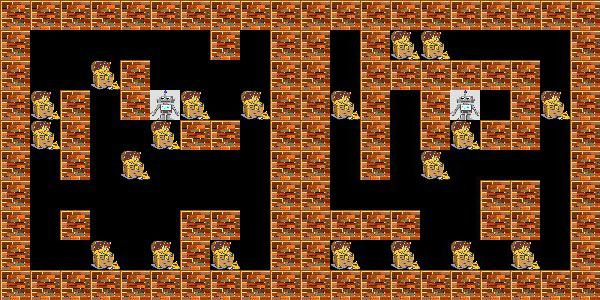
\includegraphics[scale=0.6]{combine_images.jpg} \\
	Vľavo: jednoduché bludisko, vpravo: komplikované bludisko
     \end{center}

Tieto dve mapy sú po celú dobu nemenné, a rozlišujeme ich na jednoduché a komplikované bludisko.\\
Robotovi sme určili pomerne priaznivú počiatočnú polohu. Vstupnými parametrami, ktoré sú  parametrizovateľné, sa priebeh výpočtu dá ovplyvniť v každom smere. Parametrizovať sa dajú nasledovné premenné: \\

\begin{tabular}{ll}
\hline
\textsc{Population Size} & určuje veľkosť populácie po celú dobu výpočtu \\ 
\textsc{Generations} & počet generácii \\
\textsc{Crossover}  & pravdepodobnosť kríženia  \\
\textsc{Mutation}  &  pravdepodobnosť mutácie génov  \\
\textsc{MinBound A MaxBound}  &  minimálna a maximálna dĺžka trasy robota \\ \hline
\end{tabular}

Pohyb robota na mape je reprezentovaný červenou farbou tak, že opakovaný priechod určitým miestom sposobí silnejšie červené zafarbenie. Vo výsledku teda vidno nielen kade robot prešeiel, ale či mal aj problémové miesta, na ktorých sa zacyklil.

\section{Výsledky}

Rozhodli sme sa aplikovať rôzne stratégie. Najprv sme venovali pozornosť 2 fitness funkciám, a ich výsledkom na oboch bludiskách. Ďaľším skúmaným prístupom bola rovnaká iniciálna populácia pre rôzne vstupné parametre.

\newpage

\subsection{Výsledky na základe fitness funkcií}
\textbf{1.stratégia}\\
Ako prvú sme otestovali asi najintuitívnejší prístup. Robot dostal nasledujúce ohodnotenia za svoje kroky:
\begin{itemize}
\item nenarazíš na stenu ale nenájdeš poklad : 1 bod
\item narazíš na stenu : -5 bodov
\item nájdeš poklad : 15 bodov
\end{itemize}
Táto stratégia reprezentuje to, že robota odmeníme ak nájde poklad, a potrestáme, ak narazí do steny. Aby sa po iteráciach neusadil na jednej lokálne dobrej možnosti, odmeníme ho aj za to že chodí. Pri veľmi malom pomere odmeny za poklad a chodenie však táto stratégia spôsobí neustále chodenie dookola, čo nebolo cieľom.

\noindent Túto stratégiu sme použili na oba typy máp, kde vstupné parametre boli:\\

\textsc{Population Size} = 100 \textsc{Generations} = 4000 \textsc{Crossover} = 0.7 \textsc{Mutation} = 0.3 resp. 0.4 

 
\begin{center}
  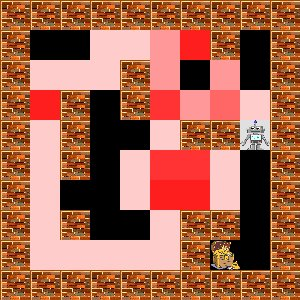
\includegraphics[scale=0.5]{strategy1_simple.jpg} 
  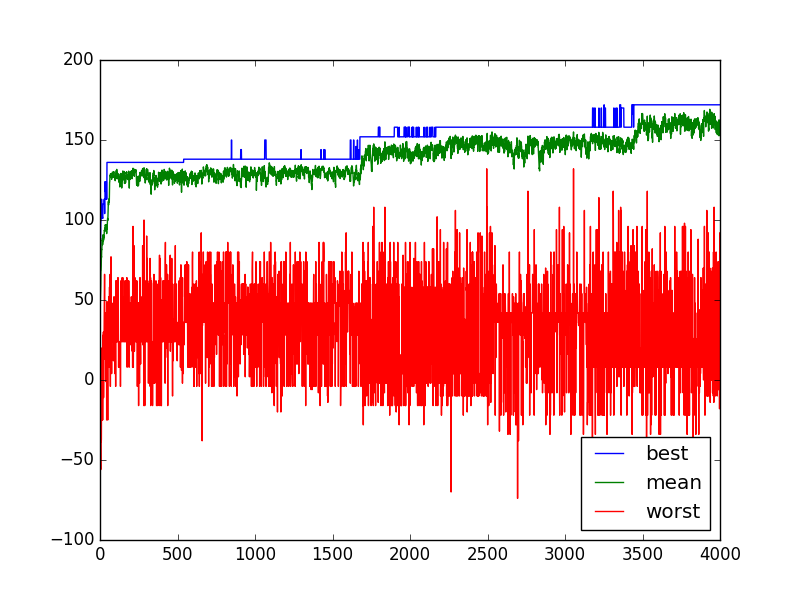
\includegraphics[scale=0.38]{strategy1_simple_graph.png} \\
   \textbf{Jednoduché bludisko}: najlepšia cesta, proces učenia
     \end{center}
     
\begin{center}
  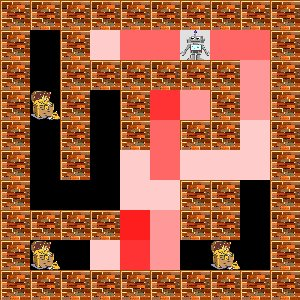
\includegraphics[scale=0.5]{strategy1_complicated.jpg} 
  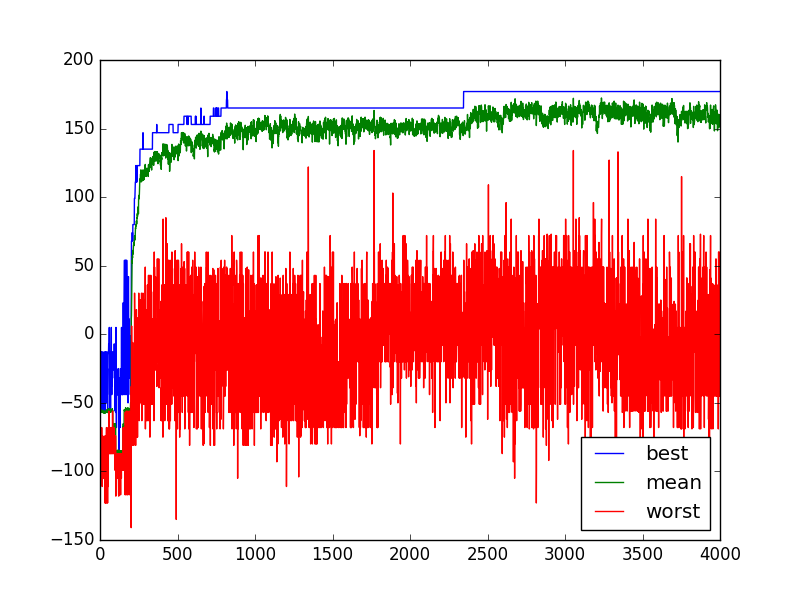
\includegraphics[scale=0.38]{strategy1_complicated_graph.png} \\
   \textbf{Kompikované bludisko}: najlepšia cesta, proces učenia
     \end{center}
     
\textit{Vyhodnotenie:} Výsledky ukazujú, že na jednoduchej mape sa bol robot schopný pomerne dobre naučiť sa nájsť poklad. Naopak, komplikované bludisko mu robilo väčšie problémy. Na kompikovanom bludisku sme skúsili aj upravené parametre, väčšiu náhodnosť mutácii, aby boli objavené iné možnosti, ako aj zvyšovanie boundu na dĺžku cesty, avšak výsledok dosiahnutý s danými parametrami považujeme za najlepší. Daná stratégia teda pre komplikované bludisko nie je vhodná. \\

\textbf{2.stratégia}\\
Ako ďaľšiu sme otestovali asi nasledovný prístup:
\begin{itemize}
\item nenarazíš na stenu ale nenájdeš poklad : 0 bodov
\item narazíš na stenu : 0 bodov
\item nájdeš poklad : 1 bod
\end{itemize}
Táto stratégia reprezentuje to, že robota odmeníme len ak nájde poklad, a teda sa predpokladá, že by sa ich mal pokúsiť nájsť čo najviac. Táto stratégia sa považuje za jednoduchšiu, a preto sme ju spustili len na 1000 iteráciach.

\noindent Túto stratégiu sme použili na oba typy máp, kde vstupné parametre boli:\\

\textsc{Population Size} = 100 \textsc{Generations} = 1000  \textsc{Crossover} = 0.6  \textsc{Mutation} = 0.4

\begin{center}
  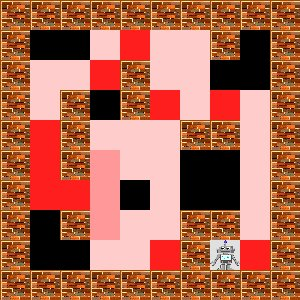
\includegraphics[scale=0.5]{strategy2_simple.jpg} 
  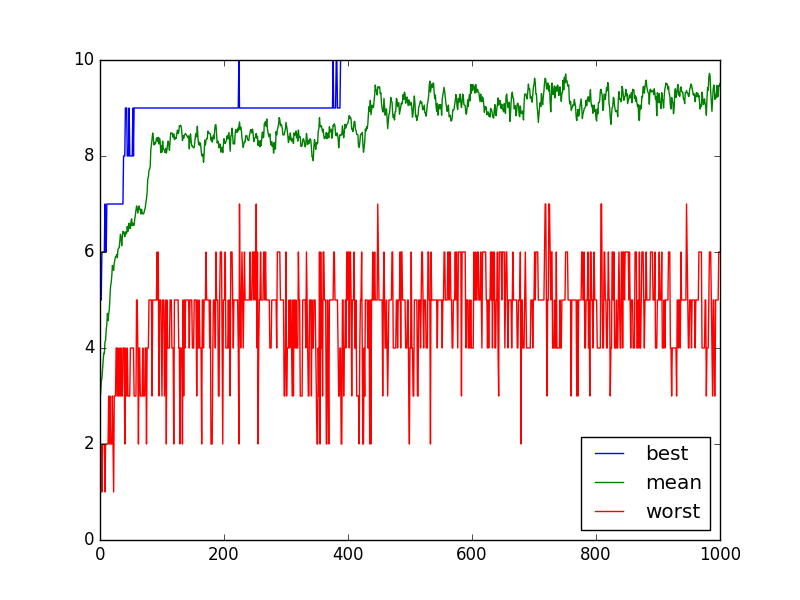
\includegraphics[scale=0.38]{strategy2_simple_graph.png} \\
   \textbf{Jednoduché bludisko}: najlepšia cesta, proces učenia
     \end{center}
     
\begin{center}
  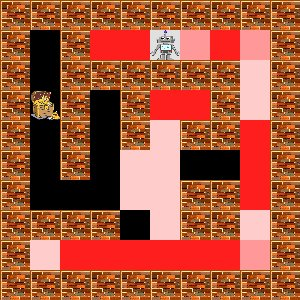
\includegraphics[scale=0.5]{strategy2_complicated.jpg} 
  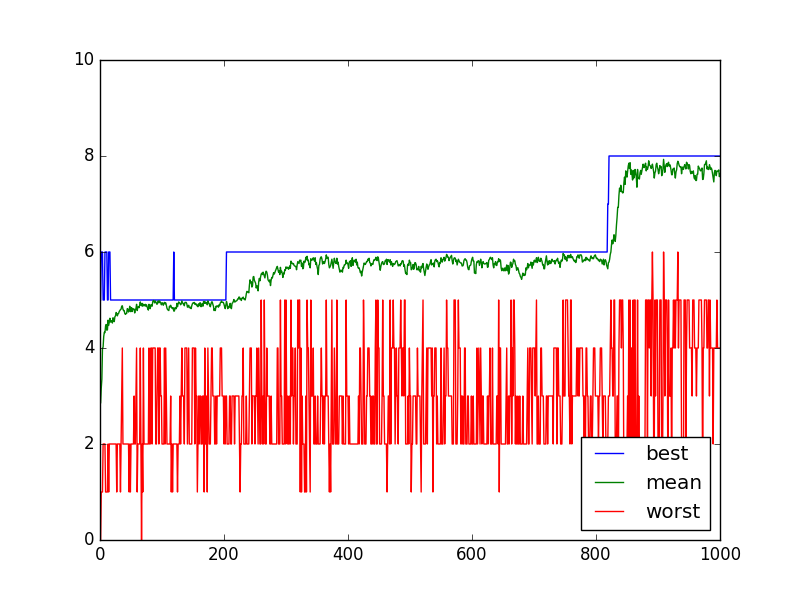
\includegraphics[scale=0.38]{strategy2_complicated_graph.png} \\
   \textbf{Kompikované bludisko}: najlepšia cesta, proces učenia
     \end{center}
     
\textit{Vyhodnotenie:} Maximálny možný počet obdov dosiahnuteľný pri tejto stratégii bol 10. Výsledky ukazujú, že robot má pre danú stratégiu dobré výsledky na oboch typoch máp. Túto stratéiu teda považujeme za veľmi efektívnu v porovnaní s jej jednoduchosťou. Ukázané výsledky predstavujú najlepší beh z 5, kde priemerné sú väčšinou o 1-2 poklady horšie.

\newpage
\subsection{Parametrizácia vstupných parametrov}

Pre obe mapy sme nagenerovali rovnaku iniciálnu populáciu a sledovali sme, ako vstupné parametre ovplyvnia dané výsledky. Minimálna a maximálna dĺžka trasy ostala po celú dobu rovnaká, tak isto ako aj veľkosť populácie. Každý beh sme spustili 4 krát a výsledky spriemerovali. 

\subsubsection{Jednoduché bludisko}

\textbf{1.stratégia}

Najprv sme testovali závislosti na kombinácii pravdepodobností kríženia a mutácie.\\
\begin{center}
\begin{tabular}{|llll|lll|}
\hline
\textsc{Population} & \textsc{Generations} & \textsc{Crossover} & \textsc{Mutation}  & best & mean & worst \\ \hline
100 & 1000 & 0.8 & 0.2 & 164.5 & 158.82 & 33.5\\ 
100 & 1000 & 0.8 & 0.4 & 170.25 & 157.24 & 66.75\\
100 & 1000 & 0.6 & 0.2 & 167.25 & 155.98 & 65.25\\
100 & 1000 & 0.6 & 0.4 & 206.75 & 178.25 & 29.0\\ \hline
\end{tabular}
\end{center}

Potom sme vybrali najúspešnejšiu stratégiu a skúmali sme ako je ovplyvnená počtom iterácií.

\begin{center}
\begin{tabular}{|llll|lll|}
\hline
\textsc{Population} & \textsc{Generations} & \textsc{Crossover} & \textsc{Mutation}  & best & mean & worst \\
100 & 100 & 0.6 & 0.4 & 154.25 &   131.84 &   37.5 \\
100 & 500 & 0.6 & 0.4 & 175.25  & 149.83 & 22.75\\
100 & 1000 & 0.6 & 0.4 & 206.75 & 178.25 & 29.0\\ 
100 & 2000 & 0.6 & 0.4 & 200.75 & 171.31 & 33.5\\
100 & 4000 & 0.6 & 0.4 & 194.25 & 167.56 & 53.5\\ \hline

\end{tabular}
\end{center}

\textbf{2. stratégia}

Najprv sme testovali závislosti na kombinácii pravdepodobností kríženia a mutácie.\\
\begin{center}
\begin{tabular}{|llll|lll|}
\hline
\textsc{Population} & \textsc{Generations} & \textsc{Crossover} & \textsc{Mutation}  & best & mean & worst \\ \hline
100 & 1000 & 0.8 & 0.2 & 7.5 & 7.36 & 4.5\\ 
100 & 1000 & 0.8 & 0.4 & 8.25 & 8.12 & 5.75\\
100 & 1000 & 0.6 & 0.2 & 9.0 & 8.56 & 4.25\\
100 & 1000 & 0.6 & 0.4 & 8.75 & 8.185 & 4.5\\ \hline
\end{tabular}
\end{center}

Potom sme vybrali najúspešnejšiu stratégiu a skúmali sme ako je ovplyvnená počtom iterácií.

\begin{center}
\begin{tabular}{|llll|lll|}
\hline
\textsc{Population} & \textsc{Generations} & \textsc{Crossover} & \textsc{Mutation}  & best & mean & worst \\
100 & 100 & 0.6 & 0.2 & 8.25 &  7.53 &  4.75 \\
100 & 500 & 0.6 & 0.2 & 8.25 & 7.92 & 4.75\\
100 & 1000 & 0.6 & 0.2 & 9.0 & 8.56 & 4.25\\ 
100 & 2000 & 0.6 & 0.2 & 9.25 & 8.97 & 4.0\\
100 & 4000 & 0.6 & 0.2 & 8.25 & 7.98 & 4.25\\ \hline
\end{tabular}
\end{center}

\textit{Vyhodnotenie:} blablablabla


\newpage 

\subsubsection{Komplikované bludisko}

\textbf{1.stratégia}

Najprv sme testovali závislosti na kombinácii pravdepodobností kríženia a mutácie.\\
\begin{center}
\begin{tabular}{|llll|lll|}
\hline
\textsc{Population} & \textsc{Generations} & \textsc{Crossover} & \textsc{Mutation}  & best & mean & worst \\ \hline

100 & 1000 & 0.8 & 0.2 & 130.5 & 126.08 & 40.25\\ 
100 & 1000 & 0.8 & 0.4 & 158.25 & 147.49 & 61.5\\
100 & 1000 & 0.6 & 0.2 & 147.0 & 137.4 & 22.25\\
100 & 1000 & 0.6 & 0.4 & 156.75 & 135.8725 & -11.75\\ \hline
\end{tabular}
\end{center}

Potom sme vybrali najúspešnejšiu stratégiu a skúmali sme ako je ovplyvnená počtom iterácií.

\begin{center}
\begin{tabular}{|llll|lll|}
\hline
\textsc{Population} & \textsc{Generations} & \textsc{Crossover} & \textsc{Mutation}  & best & mean & worst \\
 
100 & 100 & 0.8 & 0.4 & 103.5 & 87.77 & 31.55 \\
100 & 500 & 0.8 & 0.4 & 136.5 & 124.5 & 18.5\\
100 & 1000 & 0.8 & 0.4 & 158.25 & 147.49 & 61.5\\ 
100 & 2000 & 0.8 & 0.4 & 147.75 & 139.68 & 23.0\\
100 & 4000 & 0.8 & 0.4 & 167.25 & 158.38 & 68.25\\ \hline

\end{tabular}
\end{center}

\textbf{2. stratégia}

Najprv sme testovali závislosti na kombinácii pravdepodobností kríženia a mutácie.\\
\begin{center}
\begin{tabular}{|llll|lll|}
\hline
\textsc{Population} & \textsc{Generations} & \textsc{Crossover} & \textsc{Mutation}  & best & mean & worst \\ \hline

100 & 1000 & 0.8 & 0.2 & 6.5 & 6.43 & 5.25\\ 
100 & 1000 & 0.8 & 0.4 & 7.0 & 6.87 & 5.0\\
100 & 1000 & 0.6 & 0.2 & 6.5 & 6.3625 & 3.5\\
100 & 1000 & 0.6 & 0.4 & 7.5 & 7.30 & 4.5\\ \hline
\end{tabular}
\end{center}

Potom sme vybrali najúspešnejšiu stratégiu a skúmali sme ako je ovplyvnená počtom iterácií.

\begin{center}
\begin{tabular}{|llll|lll|}
\hline
\textsc{Population} & \textsc{Generations} & \textsc{Crossover} & \textsc{Mutation}  & best & mean & worst \\
100 & 100 & 0.6 & 0.2 & 6.25 & 5.95 & 3.5 \\
100 & 500 & 0.6 & 0.2 & 7.25 & 7.02 & 4.0\\
100 & 1000 & 0.6 & 0.2 & 7.5 & 7.30 & 4.5\\ 
100 & 2000 & 0.6 & 0.2 & 7.5 & 7.29 & 5.0\\
100 & 4000 & 0.6 & 0.2 & 7.5 & 7.23 & 4.25\\ \hline
\end{tabular}
\end{center}

\textit{Vyhodnotenie:} blablablabla

\section{Záverečný pokec}

Sme krásne a skvele!

\end{document}\grid
